\documentclass{article}
\usepackage[T1]{fontenc}
\usepackage[utf8]{inputenc}
\usepackage[icelandic]{babel}
\usepackage{graphicx}
\usepackage{fancyhdr}
\usepackage{listings}
\usepackage{xcolor}
\usepackage{lipsum} 
\pagestyle{fancy}
\fancyhf{}
\rhead{Vélmenni II}
\lhead{\begin{picture}(0,0) \put(0,0){
\includegraphics[width=3cm]{img/tskoli.jpg}} \end{picture}}
\lfoot{Heiti vélmennis}
\rfoot{\thepage}
\begin{document}
\title{Vélmenni II}
\author{Sveinn Máni og Vytautas}
\maketitle
\begin{figure}[h]
\centering

\includegraphics[scale=.65]{img/tskoli.jpg}
\includegraphics[scale=1]{img/rob2b3u_img.jpg}
\end{figure}
\newpage
\tableofcontents
\newpage
\section{Inngangur}
Við ákváðum að búa til eftirlits róbot. Í grunninn á vélmennið að fara hring í kringum tiltekið
svæði og taka upp allt sem verður í vegi þess. Ástæðan fyrir því að við völdum þetta verkefni
er því það er mjög sveigjanlegt og ekki flókið að fá grunn virknina til að virka. Síðan þegar
það er komið er hægt að bæta við allskonar eiginleikum sem bæta virkni vélmennisins. Þær 
hugmyndir sem við höfum fengið og munum bæta við eftir því hversu mikin tíma við höfum eru t.d.
leyfa manneskju að stýra vélmenninu með appi, láta myndavélina geta hreyfst í margar áttir,
Gera vélmenninu kleift að keyra sjálfur án þess að klessa á neitt og komast aftur á rétta braut
ef það þurfti að sveigja hjá einhverju, láta vélmennið þekkja sitt svæði og senda út viðvörun
ef hann skynjar einhverja breytingu. Mismunandi og misflóknar aðferðir við að leysa margt að
þessu sem gerir þetta að skemmtilegu og krefjandi verkefni án þess þó að enda með ekki neitt
í höndunum. \cite{cite1}
\begin{figure}[h]
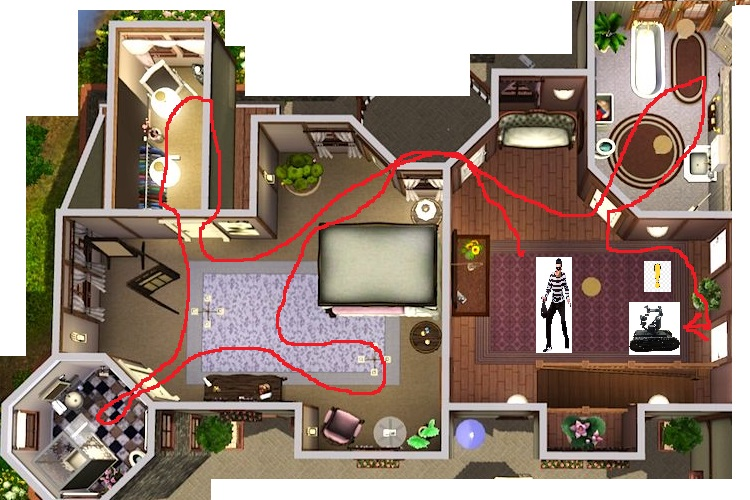
\includegraphics[scale=.4]{img/husmynd}
\end{figure}
\section{Vélbúnaður}
Hér fyrir neðan er tafla yfir allan vélbúnað sem við notuðum við verkefnið:

\begin{center}
\begin{tabular}{ |c|c|c| } 
 \hline
 Vél/rafbúnaður &Spenna &Viðnám\\ 
 Raspberry Pi 3 Model B & &\\ 
 HC-SR04 &5V &  \\ 
 Breadboard & & \\
 Vex 239 motor & 7,2V & \\
 Raspberry Pi Camera V2,1 & & \\
 Vex Shaft Encoder & 5V & \\
 \hline
\end{tabular}
\end{center}
\section{Verkáætlun}
Hér er tímaplanið okkar sett í gantt rit:
\begin{figure}[h]
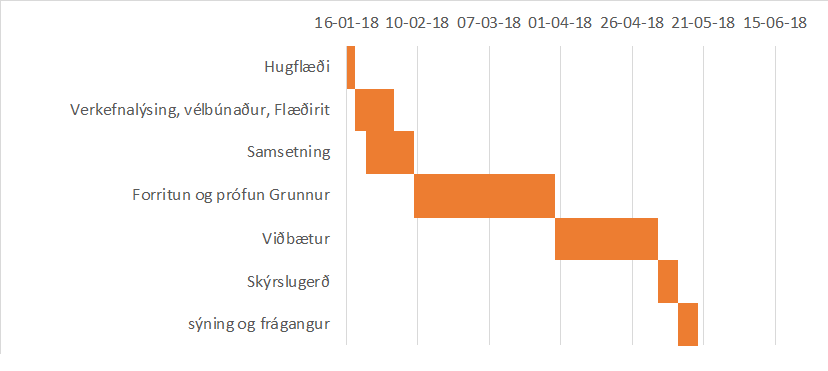
\includegraphics[scale=.7]{img/timaaetlun}
\end{figure}
\newpage
\section{Flæðirit og sauðakóði}
\begin{figure}[h]
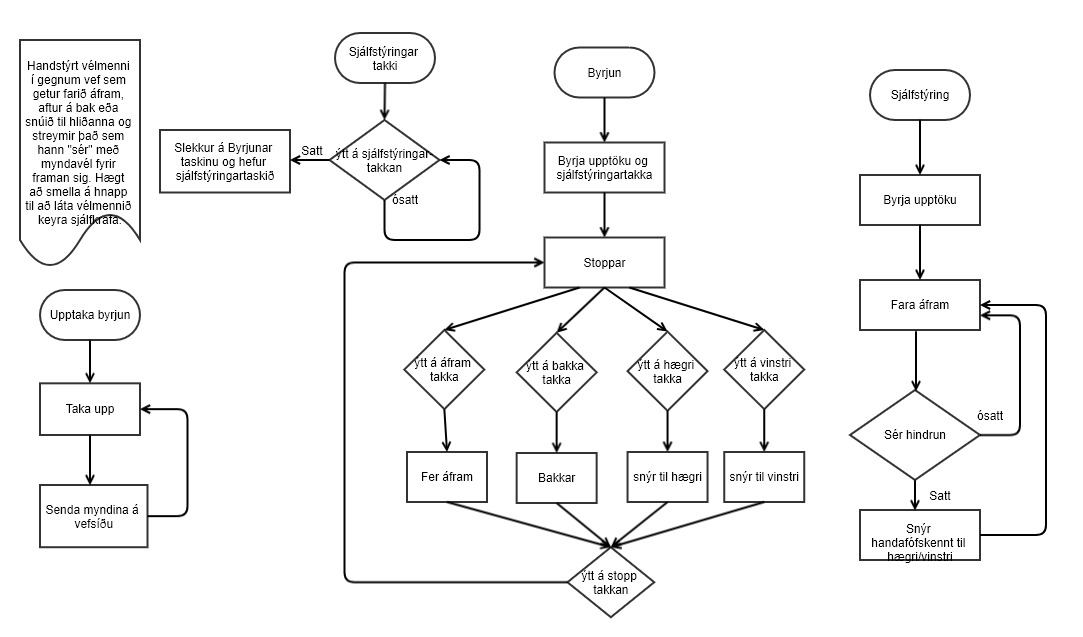
\includegraphics[scale=.3]{img/skodi}
\end{figure}

\section{Prófanir}
Áður en við byrjuðum að setja vélmennið okkar saman þá prófuðum við alla partana sem við ætluðum að nota fyrir þetta verkefni. Fyrsti parturinn sem við reyndum að fá til þess að virka var Ultrasonic sernsor sem við notum fremst á vélmenninu svo það keyri ekki á veggi. Kóðinn sem við notuðum til að athuga með sonar fengum við frá kennaranum. Við ætluðum að nota shaft encoder fyrir verkefnið og fengum það til þess að virka en hættum við að nota þá. Fengum mótora næst til þess að virka. Við notuðum H-Bridge til að stjórna þeim. Í vefhlutanum renydum við að fá takka til þess að stjórna GPIO pinnunum. Það virkaði strax með LED perum en ekki með mótorum. Erum að reyna að láta vefinn keyra console commands.  \cite{pi2015raspberry}

\section{Lokaorð}
Verkefnið gékk mjög brösulega hjá okkur aðallega útaf tæknilegra erfiðleika með py tölvuna. Hún byrjaði mjög snemma að hitna mjög mikið og undir lokin á verkefninu þá hélst hún gangandi í mjög stuttan tíma þannig við náðum ekki að taka upp lokaafraksturinn.
Annars náðum við að framkvæma þá parta af verkefninu sem við vildum fá til að virka og þó það hafi tekið sinn tíma og mismunandi aðferðir með t.d. vefinn og kóðan þá virkaði allt saman undir lokin. Við lærðum að skipuleggja og setja saman verkefni á faglegri hátt en áður og einnig fengum betri innsýn á linux kerfum sem og nota python til að stjórna GPIO pinnum.
Samvinnan í hópnun gékk mjög vel og áttum við létt með að skipta niður verkefnum en hjálpuðum þó hver öðrum þegar við lentum í mismunandi vandræðum.
Allt í allt erum við sáttir með loka útkomuna með það í huga að þetta hafði getað verið mjög flott vélmenni hefðum við ekki lent í vandræðum með tölvuna.
\newpage
\section{Heimildaskrá}

\bibliographystyle{plain}
\bibliography{mybib}
\newpage
\section{Viðauki}
\begingroup
\obeylines
\subsection{Dagbók Sveinn}
\input{dagbok_S.txt} \cite{cite3} \cite{cite4} \cite{cite6}
\subsection{Dagbók Vytautas}
\input{dagbok_V.txt} \cite{cite1} \cite{cite2} \cite{cite5} 
\endgroup
\subsection{Kóði Python}
\begingroup
\lstinputlisting[language=Python]{code/main.py} \cite{cite6}
\subsection{Kóði Index síða}
\begingroup
\lstinputlisting[language=Python]{code/index.php}
\subsection{Kóði Vefþjónn}
\begingroup
\lstinputlisting[language=Python]{code/test.txt}
\endgroup
\end{document}